\section{The Hypergeometric Distribution}
\subsection{Sampling Without Replacement and Population Formulas}

The hypergeometric distribution models the number of successes in $n$ draws \emph{without replacement} from a finite population of size $N$ that contains $K$ successes and $N-K$ failures. Its probability function is
\begin{align}
 \label{eq:2.10.11}
 f(k) = P(X=k) = \dfrac{\binom{K}{k}\binom{N-K}{n-k}}{\binom{N}{n}}, \quad \max(0, n-(N-K)) \leq k \leq \min(n, K).
\end{align}

Unlike the previous distributions, the trials here are \emph{not independent} because sampling without replacement changes the probabilities with each draw.

{Properties of the hypergeometric distribution} If $X$ has a hypergeometric distribution with parameters $N$, $K$, and $n$, then
\begin{align}
 \mu_{X} &= n\dfrac{K}{N} \\
 \s_{X}^{2} &= n\dfrac{K}{N}\dfrac{N-K}{N}\dfrac{N-n}{N-1}.
\end{align}

The factor $\dfrac{N-n}{N-1}$ is known as the \emph{finite population correction factor}. When $n \ll N$, this factor tends to $1$ and the hypergeometric distribution approaches the binomial with parameters $n$ and $p=K/N$.

\begin{ejemplo}
 \label{exmp:2.10.16}
 A batch contains $20$ items, of which $5$ are defective. If $4$ items are selected at random without replacement, what is the probability of finding exactly $2$ defective items?
\end{ejemplo}

\begin{solucion}
	Here $N=20$, $K=5$, $n=4$, $k=2$.
	\begin{align}
		P(X=2) &= \dfrac{\binom{5}{2}\binom{15}{2}}{\binom{20}{4}} \\
		&= \dfrac{10 \times 105}{4845} \\
		&= \dfrac{1050}{4845} \approx 0.2167
	\end{align}
\end{solucion}

\begin{ejemplo}
 \label{exmp:2.10.17}
 In a $5$-card poker hand dealt from a $52$-card deck, what is the probability of obtaining exactly $3$ kings?
\end{ejemplo}

\begin{solucion}
	Here $N=52$ (total cards), $K=4$ (kings), $n=5$ (cards in the hand), $k=3$.
	\begin{align}
		P(X=3) &= \dfrac{\binom{4}{3}\binom{48}{2}}{\binom{52}{5}} \\
		&= \dfrac{4 \times 1128}{2598960} \\
		&= \dfrac{4512}{2598960} \approx 0.00174
	\end{align}
\end{solucion}

\lstinputlisting[language=Python]{../code/distribuciones-especiales/distHyper.py}

\begin{figure}
 \centering
 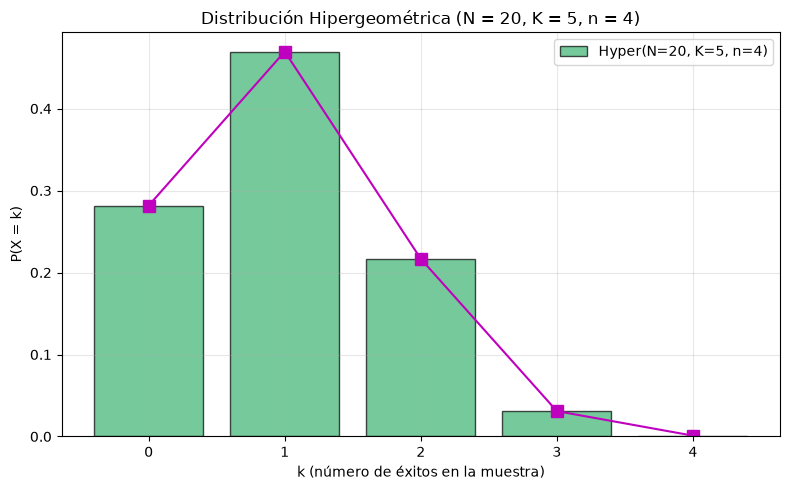
\includegraphics[height=7cm,keepaspectratio=true]{./pe/distHyper.png}
 % distHyper.png: 0x0 pixel, 300dpi, 0.00x0.00 cm, bb=
 \caption{Hypergeometric distribution with $N=20$, $K=5$, $n=4$}
 \label{fig:2.10.9}
\end{figure}

\begin{observacion}
	The hypergeometric distribution reduces to the binomial when sampling is done with replacement (or equivalently, as $N \to \infty$). In practice, if $\frac{n}{N} < 0.05$, the binomial approximation is reasonably accurate.
\end{observacion}
